% Source: https://www.dropbox.com/sh/2fx6pg4ydpu9t7x/AAAdJfzvLjeym1gJwKrIWwhBa?preview=Python+Activity+08+While+Loops+-+POGIL.docx
% File: "looping structures while loops.pdf"
% Access: 04-15-2022

% comment out for student version
% \ifdefined\Student\relax\else\def\Teacher{}\fi

\documentclass[12pt]{article}

\title{Activity \#7: While Loops}
\author{Lisa Olivieri}
\newcommand{\activityeditor}{Preston Carman}
\newcommand{\activitysource}{\url{https://www.dropbox.com/sh/2fx6pg4ydpu9t7x/AAAdJfzvLjeym1gJwKrIWwhBa?preview=Python+Activity+08+While+Loops+-+POGIL.docx}}
\date{Spring 2022}

\input{../../cspogil.sty}
\usepackage{tikz}
\usepackage{amssymb}

\begin{document}

\begin{center}
  \Large Activity \#7: While Loops \\[5pt]
  \large Recorder's Report\\[20pt]
  \normalsize
  \begin{tabular}{lrp{0.1in}lr}
      Manager:  & \ans{} &  & Reader: & \ans{}            \\[15pt]
      Recorder: & \ans{} &  & Driver: & \ans{}            \\[15pt]
      Date:     & \ans{} &  & Score:  & Satisfactory \hspace{10pt} /
      \hspace{10pt} Not Satisfactory
  \end{tabular}
\end{center}
\par\vskip 15pt

Record your team's answers to the key questions (marked with
\raisebox{-.3\height}{\includegraphics[width=0.5in]{../figures/key.png}})
below.
\begin{enumerate}[label=(\alph*)]
  \itemsep 1.25in
  \item Model 1, Question \#4
  \item Model 2, Question \#11.f
  \item Model 3, Question \#15
\end{enumerate}

\newpage
\maketitle

In this course, you will work in teams of 3--4 students to learn new concepts.
This activity will introduce you to the process of analyzing an algorithm complexity.

%\rolenames

\guide{
  \item Explain the three parts of a loop.
  \item Explain the syntax of a {\tt while} loop in C++.
  \item Explain {\bf sentinel-controlled} and {\bf counter-controlled} loops.
  \item Explain {\bf assignment operators}.
}{
  \item Write code that includes {\bf sentinel-controlled} and {\bf counter-controlled} loops.
  \item Write code that uses {\bf assignment operators}. \\[-5pt]
}{
No additional notes.
}

  
  {\bf\large Model 1: A Diagram and A C++ Code Snippet} \\[-15pt]
  \begin{center}
    \small
    \begin{tabular}{p{2in}p{3in}}
      \begin{minipage}{2in}
        \centering\par\vskip 10pt
        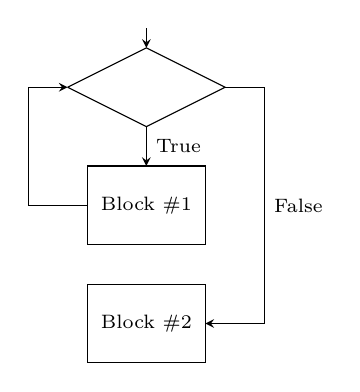
\begin{tikzpicture}
          % two rectangles
          \draw (0.25,1.5) -- (1.75,1.5) -- (1.75,2.5) -- (0.25,2.5) -- (0.25,1.5);
          \draw (0.25,0) -- (1.75,0) -- (1.75,1) -- (0.25,1) -- (0.25,0);
          % one triangle
          \draw (0,3.5) -- (1,3) -- (2,3.5) -- (1,4) -- (0,3.5);
          % five arrows
          \draw[-stealth] (1,4.25) -- (1,4);
          \draw[-stealth] (1,3) -- node[right] {\scriptsize True} (1,2.5);
          \draw[-stealth] (0.25,2) -- (-0.5,2) -- (-0.5,3.5) -- (0,3.5);
          \draw[-stealth] (2,3.5) -- (2.5,3.5) -- node[right] {\scriptsize False} (2.5,0.5) -- (1.75,0.5);
          % text
          \node[] at (1,2) {\scriptsize Block \#1};
          \node[] at (1,0.5) {\scriptsize Block \#2};
        \end{tikzpicture}
        \par\vskip 4pt\ \      
      \end{minipage}
      &
      \begin{minipage}{3in}
        \begin{minted}[
          frame=lines,
          framesep=2mm,
          bgcolor=gray!15,
          baselinestretch=1.2,
          linenos,
	  firstnumber=6
        ]{cpp}
  // print a person's name 10 times        
  string name;
  cout << "Enter your name: ";
  cin >> name;
  int x = 0;
  while (x < 10) {
    cout << name << endl;
    x = x + 1;
  }
  cout << "Nice to meet you!" << endl;
        \end{minted}
      \end{minipage}
    \end{tabular}
  \end{center}
  \TPMargin{5pt}
  
  
  {\it\large Refer to Model 1 above as your team develops consensus answers
    to the questions below.}
    \par\vskip 10pt
    
  \begin{enumerate}
    \itemsep 20pt
    
    \item Which lines of code go with the following shapes on the provided diagram?
      \par\vskip 20pt
      \begin{enumerate}[(a)]
        \itemsep 15pt
        \item The diamond \hfill 
          \fillin[Line 11 contains the condition in the diamond][4in]
        \item The ``Block \#1'' rectangle \hfill 
          \fillin[Lines 12 and 13 make up the statements in block \#1][4in]
        \item The ``Block \#2'' rectangle \hfill 
          \fillin[Line 15 contains the statement in block \#2][4in]
      \end{enumerate}
      
    \item Every loop structure requires three different actions.  Identify the line in the C++
      code snippet above that corresponds to each of these actions.
      \par\vskip 20pt
      \begin{enumerate}[(a)]
        \itemsep 15pt
        \item {\bf Initialize} a variable to control the number of loop iterations. \hfill\fillin[Line 10][1in]
        \item {\bf Test} a condition to determine if we should keep looping. \hfill\fillin[Line 11][1in]
        \item {\bf Update} the variable involved in the test condition. \hfill\fillin[Line 13][1in]
      \end{enumerate}     

\newpage

    \item The complete program is in {\tt activity07a.cpp}.  Run the program and
      answer the following questions.
      \begin{enumerate}[(a)]
        \item What would the model program do differently if line 10 was: \mintinline{cpp}|int x = 1;|?
          \begin{solution}[0.4in]
            It would only print out 9 copies of the name.
          \end{solution}
        \item What would the model program do differently if line 11 was: \mintinline{cpp}|while (x <= 10) {|?
          \begin{solution}[0.4in]          
            It would print out 11 copies of the name.
          \end{solution}
        \item What would the model program do differently if line 13 was: \mintinline{cpp}|x=x+2;|?
          \begin{solution}[0.4in]
            It would only print out 5 copies of the name.
          \end{solution}
      \end{enumerate}
      \par\vskip -40pt\null
      
    \item Change one or more of lines 10, 11, and 13 to make the program print the name 23 times.\key\\[-2.5mm]
      
      \begin{solution}[1.25in]
        \par
        Answers will vary, but one solution is to change line 6 to read:
        \begin{center}
          \mintinline{cpp}| while ( x < 23 ) {|
        \end{center}        
      \end{solution}
      
  \newpage
  \model{Another C++ Code Snippet} \\
  
  \begin{center}
    \small
    \begin{minipage}{5.5in}
      \begin{cprlst}[
        frame=lines,
        framesep=2mm,
        bgcolor=gray!15,
        baselinestretch=1.2,
        linenos,
        firstnumber=5
      ]{cpp}
  int number;
  int total = 0;
  for (int i = 0; i < 5; i += 1) {
    cout << "Enter a number: ";
    cin >> number;
    total += number;
  }
  cout << "The total is: " << total << endl;
      \end{cprlst}
    \end{minipage}
  \end{center}

  {\it\large Refer to Model 2 above as your team develops consensus answers
    to the questions below.}
    \par\vskip 5pt

    \Q The code for this program is in {\tt
      activity08b.cpp}.  Run it and explain what the program does.
      \begin{answer}[1in]
        \par
        The program prompts the user for five numbers and then prints
        out the sum of those five numbers.
      \end{answer}
      
    \Q Explain what each of the indicated lines of code from the model above does.
      \par\vskip 10pt
      \begin{enumerate}[(a)]
        \itemsep 15pt
        \item Line 6:    \hfill \ans[5.25in]{Initializes the variable {\tt total} to zero}
        \item Line 7:    \hfill \ans[5.25in]{Sets up the {\tt for} loop to repeat five times.}
        \item Line 10:   \hfill \ans[5.25in]{Adds the user-entered number to the accumulated total}
      \end{enumerate}
      
    \Q An {\it accumulator} is a variable that stores the sum of a group of values.  Which variable 
      in this model is an accumulator?  Check all that apply.
      
      \begin{checkboxes}
        \begin{multicols}{3}
          \choice {\tt number}
          \correctchoice {\tt total}
          \choice {\tt i}
        \end{multicols}
      \end{checkboxes}

    \Q Why is the variable {\tt total} initialized to zero in line 2 of the model?
      \begin{answer}[0.5in]
        \par
        Because we need to start the loop with nothing accumulated so that after the loop is
        done, total will contain just the sum of the five numbers entered.
      \end{answer}

    \Q Would it be possible to use the same variable as both a counter and an accumulator? Explain.
      \begin{answer}[0.5in]
        \par
        No.  A counter must count how many times the loop executes, so 
        it can not accumulate a sum of a group of values.
      \end{answer}

    \Q An accumulator can also store the product of a set of numbers.  How, if at all, would you \key\\[-2.5mm]
      change the following lines of the model to compute $5!$ ($5! = 1\times 2\times 3\times 4\times 5$ is called ``five factorial'').
      
      \begin{enumerate}[(a)]
        \item How would you change \cpp{int total = 0;} on line 6?
          \begin{answer}[0.5in]
            It would become \cpp{int total=1;} to initialize the accumulator to 1 instead of 0.
          \end{answer}
        \item How would you change \cpp{for (int i = 0; i < 5; i += 1)} on line 7?
          \begin{answer}[0.5in]
            This does not need to change.
          \end{answer}
        \item How would you change lines 8-9 in the model?
          \begin{answer}[0.5in]
            They would be deleted since user input is no longer needed.
          \end{answer}
        \item How would you change \cpp{total += number} on line 10 of the model?
          \begin{answer}[0.5in]
            It would become \cpp{total *= i+1} to multiply the accumulator by the counter.
          \end{answer}
      \end{enumerate}
      \par\vskip 20pt
  \newpage
   {\bf\large Model 3: Assignment Operators} \\[-10pt]
  \begin{center}
    \renewcommand{\arraystretch}{1.3}
    \begin{tabular}{|c|c|c|}
      \hline
      \rowcolor{orange!20} Initial {\tt x} Value & Assignment Operator & Final {\tt x} Value \\
      \hline
      2 & \mintinline{cpp}|x += 1;| & 3 \\
      \hline
      2 & \mintinline{cpp}|x -= 1;| & 1 \\
      \hline
      4 & \mintinline{cpp}|x *= 2;| & 8 \\
      \hline
      4 & \mintinline{cpp}|x /= 2;| & 2 \\
      \hline
      7 & \mintinline{cpp}|x %= 4;| & 3 \\
      \hline
    \end{tabular}
  \end{center}
  
  {\it\large Refer to Model 3 above as your team develops consensus answers
    to the questions below.}

    \item The code \mintinline{cpp}|x += 5;| is equivalent to which of the following lines of code?\par\vskip 10pt
      \hspace{20pt}
      \begin{oneparcheckboxes}
        \choice \mintinline{cpp}|x = 5;|
        \choice \mintinline{cpp}|x = y + 5;|
        \correctchoice \mintinline{cpp}|x = x + 5;|
        \choice \mintinline{cpp}|y = x + 5;|
      \end{oneparcheckboxes}
      
    \item An {\it assignment operator} provides a concise way of creating assignment statements when the variable on the
      left-hand side (LHS) will also appear on the right-hand side (RHS).  In your own words, describe what each of the 
      following assignment operators does.
      \par\vskip 20pt
      
      \begin{enumerate}[(a)]
        \itemsep 15pt
        \item \mintinline{cpp}|+=| \hspace{20pt} 
          \fillin[Adds the amount on the RHS to the variable on the LHS][5.25in]
        \item \mintinline{cpp}|-=| \hspace{20pt}
          \fillin[Subtracts the amount on the RHS from the variable on the LHS][5.25in]
        \item \mintinline{cpp}|*=| \hspace{20pt} 
          \fillin[Multiplies the variable on the LHS by the amount on the RHS][5.25in]
        \item \mintinline{cpp}|/=| \hspace{20pt} 
          \fillin[Divides the variable on the LHS by the amount on the RHS][5.25in]
        \item \mintinline{cpp}|%=| \hspace{20pt} 
          \fillin[Adds the amount on the RHS to the variable on the LHS][5in]
      \end{enumerate}
      
\newpage

    \item The table below is similar to that seen in Model 3.  Fill in the missing pieces with appropriate values or
      assignment operator statements.  Assume that {\tt x} is an integer variable.
      
      \begin{center}
        \renewcommand{\arraystretch}{1.5}
        \begin{tabular}{|c|c|c|c|}
          \hline
          \rowcolor{orange!20} Operator & Initial {\tt x} Value & Statement & Final {\tt x} Value \\
          \hline
          \mintinline{cpp}|+=| & 6 & \ifprintanswers\mintinline{cpp}|x += 1;|\fi & 8 \\
          \hline
          \mintinline{cpp}|+=| & 5 & \mintinline{cpp}|x -= x+1;| & \ifprintanswers 11\fi \\
          \hline
          \mintinline{cpp}|-=| & \ifprintanswers 9\fi  & \mintinline{cpp}|x -= 3;| & 6 \\
          \hline
          \mintinline{cpp}|*=| & 4 & \ifprintanswers\mintinline{cpp}|x *= 4;|\fi & 4 \\
          \hline
          \mintinline{cpp}|/=| & 23 & \ifprintanswers\mintinline{cpp}|x /= 10;|\fi & 2 \\
          \hline
        \end{tabular}
      \end{center}
      \par\vskip -40pt\null
      
    \item Is the assignment operator \mintinline{cpp}|23 += total|
    valid?  Why or why not?\key
      \begin{solution}[0.5in]
        No, it is not valid.  There must be only a variable name on the left-hand side.
      \end{solution}
      
    \item The following code snippet should print the numbers beginning with 100 and counting down to 1.  However, it is missing a
      line of code.  Add the missing code using an assignment operator.  Indicate the line number at which the code should be inserted.
      \par\vskip 10pt
      \begin{tabular}{p{2.4in}p{3.4in}}
        \begin{minipage}{2.4in}
          \begin{minted}[
            frame=lines,
            framesep=2mm,
            bgcolor=gray!15,
            baselinestretch=1.2,
            linenos
          ]{cpp}
  int countdown = 100;
  while (countdown > 0) {
    cout << countdown << endl;
  }
          \end{minted}
          \par\vskip 10pt\null
        \end{minipage}
        &
        \begin{minipage}{3.4in}
          \begin{solution}[0.5in]
            \par
            Insert the command \mintinline{cpp}|x -= 1;| between lines 3 and 4.
          \end{solution}            
        \end{minipage}
      \end{tabular}
      \par\vskip -40pt\null
      
    \item Use assignment operators to write loops to do each of the following.  
      You can test your code in the {\tt activity07c.cpp} file.
      
      \begin{enumerate}[(a)]
        \item A loop that prints out all multiples of three between 0 and 100. (i.e. 0, 3, 6, 9, {\ldots} )
          \begin{solution}[1.5in]
            \begin{center}
              \scriptsize
              \begin{minipage}{3in}
                \begin{minted}[
                  frame=lines,
                  framesep=2mm,
                  bgcolor=gray!15,
                  baselinestretch=1.2,
                  linenos
                ]{cpp}
  int num = 0;
  while (num <= 100) {
    cout << num << endl;
    num += 3;
  }
                \end{minted}
              \end{minipage}
            \end{center}
          \end{solution}
        \item A loop that prints all powers of 2 (i.e. $2^n$) from 1 up to 100.
          \begin{solution}[1.5in]
            \begin{center}
              \scriptsize
              \begin{minipage}{3in}
                \begin{minted}[
                  frame=lines,
                  framesep=2mm,
                  bgcolor=gray!15,
                  baselinestretch=1.2,
                  linenos
                ]{cpp}
  int num = 1;
  while (num <= 100) {
    cout << num << endl;
    num *= 2;
  }
                \end{minted} 
              \end{minipage}
           \end{center}              
          \end{solution}
      \end{enumerate}

  \end{enumerate}  
    
\end{document}
